\chapter{Specifikacija programske potpore}
		
	\section{Funkcionalni zahtjevi}
			
			\noindent \textbf{Dionici:}
			
			\begin{packed_enum}
				
				\item Vlasnik životinje
				\item Tvrtka				
				\item Administrator
				\item Razvojni tim
				
			\end{packed_enum}
			
			\noindent \textbf{Aktori i njihovi funkcionalni zahtjevi:}
			
			
			\begin{packed_enum}
				\item  \underbar{Neregistrirani/neprijavljeni korisnik može:}
				
				\begin{packed_enum}
					
					\item Pregledavati početnu stranicu platforme Naši ljubimci.
					\item Registrirati se na platformu Naši ljubimci.
					
				\end{packed_enum}
			
				\item  \underbar{Prijavljeni korisnik, vlasnik životinje može:}
				
				\begin{packed_enum}
					
					\item Uređivati vlastiti korisnički profil.
					\item Kreirati profil za svojeg ljubimca.
					\item Uređivati profil ljubimca.
					\item Objavljivati foto I video materijale uz kratki opis na profilu svojega ljubimca.
					\item Objavljivati foto I video materijale uz kratki opis u medijskim galerijama vlastitih profila.
					\item Komentirati na medijskim galerijama profila drugih vlasnika ljubimaca.
					\item Komentirati objevljene sadržaje na profilu tvrtki.
					\item Slati zahtjeve za prijateljstvo.
					\item Prihvatiti ili odbiti zahtjev za prijateljstvo ili pak trajno blokirati pošiljatelja zahtjeva. 
					\item Kreirati događaje.
					\item Navesti status uz sebi vidljive događaje.
					\item Pretraživati korisnike.
					\item Slati izravne poruke.
					\item Prijaviti korisnika administratoru.
					
				\end{packed_enum}
			
				\item  \underbar{Prijavljeni korisnik, tvrtka može:}
				
				\begin{packed_enum}
					
					\item Objavljivati kratke poruke, foto I video materijale na vlastitom profilu.
					\item Kreirati nove događaje.
					\item Slati izravne poruke.
					
				\end{packed_enum}
			
				\item  \underbar{Administrator može:}
				
				\begin{packed_enum}
					
					\item Privremeno blokirati registriranog korisnika, vlasnika ili tvrtku.
					\item Trajno izbrisati korisnički račun. 
					
				\end{packed_enum}
				
			\end{packed_enum}
			
			\eject 
			
			
				
			\subsection{Obrasci uporabe}
				
				
				\subsubsection{Opis obrazaca uporabe}

					\noindent \underbar{\textbf{UC1 - Pregled stranice}}
					\begin{packed_item}
	
						\item \textbf{Glavni sudionik: } Korisnik
						\item  \textbf{Cilj:} Pregled stranice Naši ljubimci
						\item  \textbf{Sudionici:} Baza podataka
						\item  \textbf{Preduvjet:} -
						\item  \textbf{Opis osnovnog tijeka:}
						
						\item[] \begin{packed_enum}
	
							\item Neregistrirani ili neprijavljeni korisnik u web pregledniku pregledava stranicu platforme Naši ljubimci 
			
						\end{packed_enum}
						
					\end{packed_item}
				
				\noindent \underbar{\textbf{UC2 - Registracija, vlasnik}}
				\begin{packed_item}
					
					\item \textbf{Glavni sudionik: } Korisnik
					\item  \textbf{Cilj:} Registracija na platformi Naši ljubimci
					\item  \textbf{Sudionici:} Baza podataka
					\item  \textbf{Preduvjet:} -
					\item  \textbf{Opis osnovnog tijeka:}
					
					\item[] \begin{packed_enum}
						
						\item Unos registracijskih podataka (ime, prezime, e-mail adresa, korisničko ime)
						\item Potvrda o ispravnosti unesenih podataka
						\item Spremanje podataka u bazu podataka
						\item Pristup korisničkim funkcijama
					\end{packed_enum}
					
					\item  \textbf{Opis mogućih odstupanja:}
					
					\item[] \begin{packed_item}
						
						\item[2.a] Zauzeto korisničko ime/e-mail
						\item[] \begin{packed_enum}
							\item Sustav obavještava korisnika o neuspjeloj registraciji i vraća  ga na stranicu za unos registracijskih podataka
							
						\end{packed_enum}
						
					\end{packed_item}
				\end{packed_item}
				
				\noindent \underbar{\textbf{UC3 - Registracija, tvrtka}}
				\begin{packed_item}
					
					\item \textbf{Glavni sudionik: } Korisnik
					\item  \textbf{Cilj:} Registracija na platformi Naši ljubimci
					\item  \textbf{Sudionici:} Baza podataka
					\item  \textbf{Preduvjet:} -
					\item  \textbf{Opis osnovnog tijeka:}
					
					\item[] \begin{packed_enum}
						
						\item Unos registracijskih podataka (ime, prezime, e-mail adresa, korisničko ime)
						\item Potvrda o ispravnosti unesenih podataka
						\item Spremanje podataka u bazu podataka
						\item Pristup korisničkim funkcijama
					\end{packed_enum}
					
					\item  \textbf{Opis mogućih odstupanja:}
					
					\item[] \begin{packed_item}
						
						\item[2.a] Zauzeto korisničko ime/e-mail
						\item[] \begin{packed_enum}
							
							\item Sustav obavještava korisnika o neuspjeloj registraciji i vraća  ga na stranicu za unos registracijskih podataka
							
						\end{packed_enum}
						
					\end{packed_item}
				\end{packed_item}
				
				\noindent \underbar{\textbf{UC4 - Prijava}}
				\begin{packed_item}
					
					\item \textbf{Glavni sudionik: } Vlasnik, tvrtka
					\item  \textbf{Cilj:} Prijava na platformi Naši ljubimci
					\item  \textbf{Sudionici:} Baza podataka
					\item  \textbf{Preduvjet:} Registracija na platformi Naši ljubimci 
					\item  \textbf{Opis osnovnog tijeka:}
					
					\item[] \begin{packed_enum}
						
						\item Unos korisničkog imena i lozinke
						\item Potvrda o ispravnosti korisničkih podataka
						\item Pristup korisničkim funkcijama
						
					\end{packed_enum}
					
					\item  \textbf{Opis mogućih odstupanja:}
					
					\item[] \begin{packed_item}
						
						\item[2.a] Neispravno korisničko ime/lozinka
						\item[] \begin{packed_enum}
							
							\item Sustav obavještava korisnika o neuspjeloj prijavi i vraća ga na 		stranicu za unos korisničkog imena i lozinke	
							
						\end{packed_enum}	
					\end{packed_item}
				\end{packed_item}
				
				\noindent \underbar{\textbf{UC5 - Uređivanje profila, vlasnik}}
				\begin{packed_item}
					
					\item \textbf{Glavni sudionik: } Vlasnik 
					\item  \textbf{Cilj:} Izmjena korisničkog profila
					\item  \textbf{Sudionici:} Baza podataka
					\item  \textbf{Preduvjet:} Prijava u sustav
					\item  \textbf{Opis osnovnog tijeka:}
					
					\item[] \begin{packed_enum}
						
						\item Korisnik odabire opciju za uređivanje profila
						\item Otvara se stranica za mijenjanje osobnih podataka
						\item Korisnik mijenja željene podatke
						\item Korisnik sprema promjene
						\item Baza podataka se ažurira
					\end{packed_enum}
					
					\item  \textbf{Opis mogućih odstupanja:}
					
					\item[] \begin{packed_item}
						
						\item[3.a] Korisnik promijeni svoje osobne podatke, ali ne odabere opciju za spremanje promjena
						\item[] \begin{packed_enum}
							
							\item Sustav obavještava korisnika da nije spremio podatke prije izlaska iz prozora
							
						\end{packed_enum}
					\end{packed_item}
				\end{packed_item}
				
				\noindent \underbar{\textbf{UC6 - Uređivanje profila, tvrka}}
				\begin{packed_item}
					
					\item \textbf{Glavni sudionik: } Tvrtka
						\item  \textbf{Cilj:} Izmjena korisničkog profila
					\item  \textbf{Sudionici:} Baza podataka
					\item  \textbf{Preduvjet:} Prijava u sustav
					\item  \textbf{Opis osnovnog tijeka:}
					
					\item[] \begin{packed_enum}
						
						\item Korisnik odabire opciju za uređivanje profila
						\item Otvara se stranica za mijenjanje osobnih podataka
						\item Korisnik mijenja željene podatke
						\item Korisnik sprema promjene
						\item Baza podataka se ažurira
					\end{packed_enum}
					
					\item  \textbf{Opis mogućih odstupanja:}
					
					\item[] \begin{packed_item}
						
						\item[3.a] Korisnik promijeni svoje osobne podatke, ali ne odabere opciju za spremanje promjena
						\item[] \begin{packed_enum}
							
							\item Sustav obavještava korisnika da nije spremio podatke prije izlaska iz prozora
							
						\end{packed_enum}
					\end{packed_item}
				\end{packed_item}
				
				\noindent \underbar{\textbf{UC7 - Stvaranje profila ljubimca}}
				\begin{packed_item}
					
					\item \textbf{Glavni sudionik: } Vlasnik
					\item  \textbf{Cilj:} Stvaranje profila ljubimca
					\item  \textbf{Sudionici:} Baza podataka
					\item  \textbf{Preduvjet:} Prijava u sustav
					\item  \textbf{Opis osnovnog tijeka:}
					
					\item[] \begin{packed_enum}
						
						\item Korisnik u aplikaciji odabire ”Dodaj ljubimca”
						\item Otvara se obrazac za popunjavanje informacija o ljubimcu
						\item Korisnik predaje obrazac
						\item Baza podataka se ažurira
						
					\end{packed_enum}
					
					\item  \textbf{Opis mogućih odstupanja:}
					
					\item[] \begin{packed_item}
						
						\item[3.a] Korisnik predaje obrazac koji nije u potpunosti ispunjen
						\item[] \begin{packed_enum}
							
							\item Sustav obavještava korisnika da mora ispuniti obrazac prije predaje
							
						\end{packed_enum}					
					\end{packed_item}
				\end{packed_item}
				
				\noindent \underbar{\textbf{UC8 - Uređivanje profila ljubimca}}
				\begin{packed_item}
					
					\item \textbf{Glavni sudionik: } Vlasnik
					\item  \textbf{Cilj:} Izmjena profilnih podataka
					\item  \textbf{Sudionici:} Baza podataka
					\item  \textbf{Preduvjet:} Prijava u sustav
					\item  \textbf{Opis osnovnog tijeka:}
					
					\item[] \begin{packed_enum}
						
						\item Korisnik odabire opciju za uređivanje profila na stranici ljubimca
						\item Otvara se stranica za mijenjanje podataka ljubimca
						\item Korisnik mijenja željene podatke
						\item Korisnik sprema promjene
						\item Baza podataka se ažurira
					\end{packed_enum}
					
					\item  \textbf{Opis mogućih odstupanja:}
					
					\item[] \begin{packed_item}
						
						\item[3.a] Korisnik promijeni svoje osobne podatke, ali ne odabere opciju za spremanje promjena
						\item[] \begin{packed_enum}
							
							\item Sustav obavještava korisnika da nije spremio podatke prije izlaska iz prozora							
							
						\end{packed_enum}						
					\end{packed_item}
				\end{packed_item}
				
				\noindent \underbar{\textbf{UC9 - Uređivanje profila ljubimca}}
				\begin{packed_item}
					
					\item \textbf{Glavni sudionik: } Vlasnik
					\item  \textbf{Cilj:} Objava foto ili video materijala 
					\item  \textbf{Sudionici:} Baza podataka
					\item  \textbf{Preduvjet:} Prijava u sustav
					\item  \textbf{Opis osnovnog tijeka:}
					
					\item[] \begin{packed_enum}
						
						\item Korisnik odabire opciju dodavanja medijskog sadržaja 
						\item Otvara se stranica za dodavanje videa ili fotografija
						\item Korisnik dodaje video ili fotografiju
						\item Korisnik sprema promjene
						\item Baza podataka se ažurira
					\end{packed_enum}
					
					\item  \textbf{Opis mogućih odstupanja:}
					
					\item[] \begin{packed_item}
						
						\item[3.a] Korisnik dodaje sadržaj, ali ne odabere opciju za spremanje promjena
						\item[] \begin{packed_enum}
							
							\item Sustav obavještava korisnika da nije spremio podatke prije izlaska iz prozora
							
						\end{packed_enum}						
					\end{packed_item}
				\end{packed_item}
				
				\noindent \underbar{\textbf{UC10 - Osobni profil, objava foto i video materijala}}
				\begin{packed_item}
					
					\item \textbf{Glavni sudionik: } Vlasnik, tvrtka
					\item  \textbf{Cilj:} Objava kratkih poruka, foto ili video materijala 
					\item  \textbf{Sudionici:} Baza podataka
					\item  \textbf{Preduvjet:} Prijava u sustav
					\item  \textbf{Opis osnovnog tijeka:}
					
					\item[] \begin{packed_enum}
						
						\item Korisnik odabire opciju dodavanja medijskog sadržaja 
						\item Otvara se stranica za dodavanje videa ili fotografija
						\item Korisnik dodaje video ili fotografiju
						\item Korisnik sprema promjene
						\item Baza podataka se ažurira
					\end{packed_enum}
					
					\item  \textbf{Opis mogućih odstupanja:}
					
					\item[] \begin{packed_item}
						
						\item[3.a] Korisnik dodaje sadržaj, ali ne odabere opciju za spremanje promjena
						\item[] \begin{packed_enum}
							
							\item Sustav obavještava korisnika da nije spremio podatke prije izlaska iz prozora
							
						\end{packed_enum}
					\end{packed_item}
				\end{packed_item}
			
				
				\noindent \underbar{\textbf{UC11 - Komentiranje na profilu tvrtke}}
				\begin{packed_item}
					
					\item \textbf{Glavni sudionik: } Vlasnik
					\item  \textbf{Cilj:} Komentiranje objavljenih sadržaja na profilu tvrtke
					\item  \textbf{Sudionici:} Baza podataka
					\item  \textbf{Preduvjet:} Prijava u sustav
					\item  \textbf{Opis osnovnog tijeka:}
					
					\item[] \begin{packed_enum}
						
						\item Korisnik odabire opciju dodavanja komentara na sadržaj
						\item Otvara se prozor za upisivanje komentara
						\item Korisnik upisuje komentar
						\item Korisnik sprema promjene
						\item Baza podataka se ažurira
					\end{packed_enum}
					
					\item  \textbf{Opis mogućih odstupanja:}
					
					\item[] \begin{packed_item}
						
						\item[3.a] Korisnik upisuje komentar, ali ne odabere opciju za objavu
						\item[] \begin{packed_enum}
							
							\item Sustav obavještava korisnika da komentar pri promjeni stranice neće biti spremljen
							
						\end{packed_enum}
						
					\end{packed_item}
				\end{packed_item}
				
				\noindent \underbar{\textbf{UC12 - Slanje zahtjeva za prijateljstvo}}
				\begin{packed_item}
					
					\item \textbf{Glavni sudionik: } Vlasnik
					\item  \textbf{Cilj:} Slanje zahtjeva za prijateljsvo drugim vlasnicima
					\item  \textbf{Sudionici:} Baza podataka
					\item  \textbf{Preduvjet:} Prijava u sustav
					\item  \textbf{Opis osnovnog tijeka:}
					
					\item[] \begin{packed_enum}
						
						\item Korisnik otvara profil drugog korisnika 
						\item Korisnik pritisne gumb ”Dodaj prijatelja”
						\item Baza podataka se ažurira
					\end{packed_enum}
					
					\item  \textbf{Opis mogućih odstupanja:}
					
					\item[] \begin{packed_item}
						
						\item[2.a] Drugi korisnik odgovara na zahtjev za prijateljstvo
						\item[] \begin{packed_enum}
							
							\item Korisnik odgovara s "Prihvati zahtjev"
							\item Korisnik odgovara s "Odbij zahtjev"
							\item Korisnik odgovara s "Blokiraj"
							
						\end{packed_enum}
					\end{packed_item}
				\end{packed_item}
				
				\noindent \underbar{\textbf{UC13 - Komentiranje u medijskoj galeriji}}
				\begin{packed_item}
					
					\item \textbf{Glavni sudionik: } Vlasnik
					\item  \textbf{Cilj:} Objava kratkog komentara u medijskoj galeriji
					\item  \textbf{Sudionici:} Baza podataka
					\item  \textbf{Preduvjet:} Prijava u sustav, prijateljsvo s vlasnikom pripadne medijske galerije
					\item  \textbf{Opis osnovnog tijeka:}
					
					\item[] \begin{packed_enum}
						
						\item Korisnik odabire opciju dodavanja komentara na sadržaj
						\item Otvara se prozor za upisivanje komentara
						\item Korisnik upisuje komentar
						\item Korisnik sprema promjene
						\item Baza podataka se ažurira
					\end{packed_enum}
					
					\item  \textbf{Opis mogućih odstupanja:}
					
					\item[] \begin{packed_item}
						
						\item[3.a] Korisnik upisuje komentar, ali ne odabere opciju za objavu
						\item[] \begin{packed_enum}
							
							\item Sustav obavještava korisnika da komentar pri promjeni stranice neće biti objavljen
							
						\end{packed_enum}
						
					\end{packed_item}
				\end{packed_item}
				
				\noindent \underbar{\textbf{UC14 - Brisanje komentara}}
				\begin{packed_item}
					
					\item \textbf{Glavni sudionik: } Vlasnik
					\item  \textbf{Cilj:} Brisanje neželjenih komentara
					\item  \textbf{Sudionici:} Baza podataka
					\item  \textbf{Preduvjet:} Prijava u sustav
					\item  \textbf{Opis osnovnog tijeka:}
					
					\item[] \begin{packed_enum}
						
						\item Korisnik odabire željeni komentar
						\item Korisnik odabire brisanje komentara
						\item Baza podataka se ažurira
					\end{packed_enum}
					
				\end{packed_item}
				
				\noindent \underbar{\textbf{UC15 - Raskid prijateljstva}}
				\begin{packed_item}
					
					\item \textbf{Glavni sudionik: } Vlasnik
					\item  \textbf{Cilj:} Raskid prijateljstva  s drugim vlasnikom
					\item  \textbf{Sudionici:} Baza podataka
					\item  \textbf{Preduvjet:} Prijava u sustav, uspostavljeno prijateljstvo s drugim vlasnikom
					\item  \textbf{Opis osnovnog tijeka:}
					
					\item[] \begin{packed_enum}
						
						\item Korisnik odabire drugoga korisnika 
						\item Korisnik odabire raskid prijateljstva 
						\item Baza podataka se ažurira
					\end{packed_enum}
					
				\end{packed_item}
				
				\noindent \underbar{\textbf{UC16 - Kreiranje događaja}}
				\begin{packed_item}
					
					\item \textbf{Glavni sudionik: } Vlasnik, tvrtka
					\item  \textbf{Cilj:} Kreiranje događaja
					\item  \textbf{Sudionici:} Baza podataka
					\item  \textbf{Preduvjet:} Prijava u sustav
					\item  \textbf{Opis osnovnog tijeka:}
					
					\item[] \begin{packed_enum}
						
						\item Korisnik odabire opciju kreiranja događaja
						\item Otvara se obrazac za popunjavanje informacija o događaju
						\item Korisnik predaje obrazac
						\item Baza podataka se ažurira
					\end{packed_enum}
					
					\item  \textbf{Opis mogućih odstupanja:}
					
					\item[] \begin{packed_item}
						
						\item[3.a] Već postoji događaj s istim sadržajem
						\item[] \begin{packed_enum}
							
							\item Sustav obavještava korisnika o već postojećem događaju i vraća ga na popunjavanje obrasca
							
						\end{packed_enum}
					\end{packed_item}
				\end{packed_item}
			
				\noindent \underbar{\textbf{UC17 - Pretraživanje}}
				\begin{packed_item}
					
					\item \textbf{Glavni sudionik: } Vlasnik  
					\item  \textbf{Cilj:} Pretraga drugih korisnika
					\item  \textbf{Sudionici:} Baza podataka
					\item  \textbf{Preduvjet:} Prijava u sustav
					\item  \textbf{Opis osnovnog tijeka:}
					
					\item[] \begin{packed_enum}
						
						\item Korisnik odabire opciju pretraživanja
						\item Korisnik upisuje ime korisnika ili tvrtke koju želi pronaći
						\item Prikazuju se rezultati pretrage
					\end{packed_enum}
					
					\item  \textbf{Opis mogućih odstupanja:}
					
					\item[] \begin{packed_item}
						
						\item[2.a] Ne postoji korisnik ili tvrtka pod tim imenom
						\item[] \begin{packed_enum}
							
							\item Sustav obavještava korisnika da nema rezultata takve pretrage
							
						\end{packed_enum}
						
					\end{packed_item}
				\end{packed_item}	
				
				\noindent \underbar{\textbf{UC18 - Prijava na događaj}}
				\begin{packed_item}
					
					\item \textbf{Glavni sudionik: } Vlasnik
					\item  \textbf{Cilj:} Navođenje statusa uz događaj
					\item  \textbf{Sudionici:} Baza podataka
					\item  \textbf{Preduvjet:} Prijava u sustav, vidljivost događaja
					\item  \textbf{Opis osnovnog tijeka:}
					
					\item[] \begin{packed_enum}
						
						\item Korisnik odabire željeni događaj
						\item Korisnik odabire jednu od opcija dolaska na događaj
						\item Baza podataka se ažurira

					\end{packed_enum}
					
					\item  \textbf{Opis mogućih odstupanja:}
					
				\end{packed_item}
				
				
				\noindent \underbar{\textbf{UC19 - Slanje poruke}}
				\begin{packed_item}
					
					\item \textbf{Glavni sudionik: } Vlasnik
					\item  \textbf{Cilj:} Slanje direktne poruke	
					\item  \textbf{Sudionici:} Baza podataka
					\item  \textbf{Preduvjet:} Prijava u sustav
					\item  \textbf{Opis osnovnog tijeka:}
					
					\item[] \begin{packed_enum}
						
						\item Korisnik se pozicionira na profil drugog korisnika 
						\item Korisnik odabire opciju ”Poruka”
						\item Korisnik upisuje željenu poruku
						\item Korisnik odabire ”Slanje poruke”
						\item Baza podataka se ažurira
					\end{packed_enum}
					
				\end{packed_item}
				
				\noindent \underbar{\textbf{UC20 - Prijava}}
				\begin{packed_item}
					
					\item \textbf{Glavni sudionik: } Vlasnik
					\item  \textbf{Cilj:} Prijava drugog korisnika ili tvrtke
					\item  \textbf{Sudionici:} Baza podataka
					\item  \textbf{Preduvjet:} Prijava u sustav
					\item  \textbf{Opis osnovnog tijeka:}
					
					\item[] \begin{packed_enum}
						
						\item Korisnik se pozicionira na profil drugog korisnika
						\item Korisnik odabire opciju ”Prijavi”
						\item Baza podataka se ažurira
					\end{packed_enum}
					
				\end{packed_item}
				
				\noindent \underbar{\textbf{UC21 - Privremeno blokiranje}}
				\begin{packed_item}
					
					\item \textbf{Glavni sudionik: } Administrator
					\item  \textbf{Cilj:} Prijava drugog korisnika ili tvrtke
					\item  \textbf{Sudionici:} Baza podataka
					\item  \textbf{Preduvjet:} Prijava u sustav
					\item  \textbf{Opis osnovnog tijeka:}
					
					\item[] \begin{packed_enum}
						
						\item Administrator pronalazi željenog korisnika
						\item Administrator odabire opciju ”Privremeno blokiraj”
						\item Baza podataka se ažurira
					\end{packed_enum}
					
				\end{packed_item}
				
				\noindent \underbar{\textbf{UC22 - Trajno brisanje}}
				\begin{packed_item}
					
					\item \textbf{Glavni sudionik: } Administrator
					\item  \textbf{Cilj:} Brisanje računa vlasnika ili tvrtke
					\item  \textbf{Sudionici:} Baza podataka
					\item  \textbf{Preduvjet:} Prijava u sustav
					\item  \textbf{Opis osnovnog tijeka:}
					
					\item[] \begin{packed_enum}
						
						\item Administrator pronalazi željenog korisnika
						\item Administrator odabire opciju ”Obriši korisnika”
						\item Baza podataka se ažurira
					\end{packed_enum}
				\end{packed_item}
						
				\subsubsection{Dijagrami obrazaca uporabe}
					\begin{figure} 
						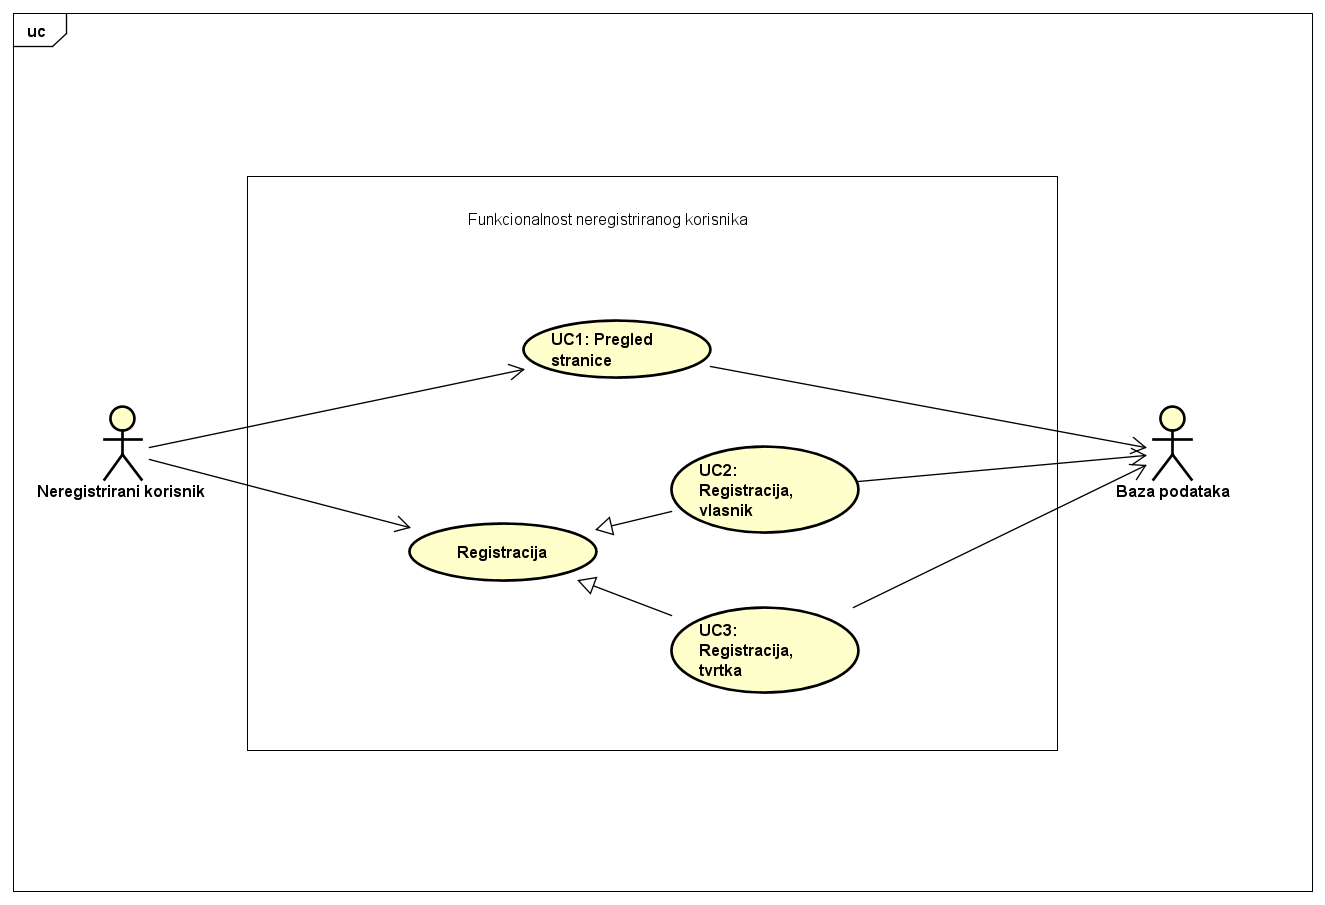
\includegraphics[width=\textwidth]{slike/funkc_neregistriranog_korisnika.png}
						\caption{Funkcionalnost neregistriranog korisnika u aplikaciji}
					\end{figure}
					\begin{figure} 
						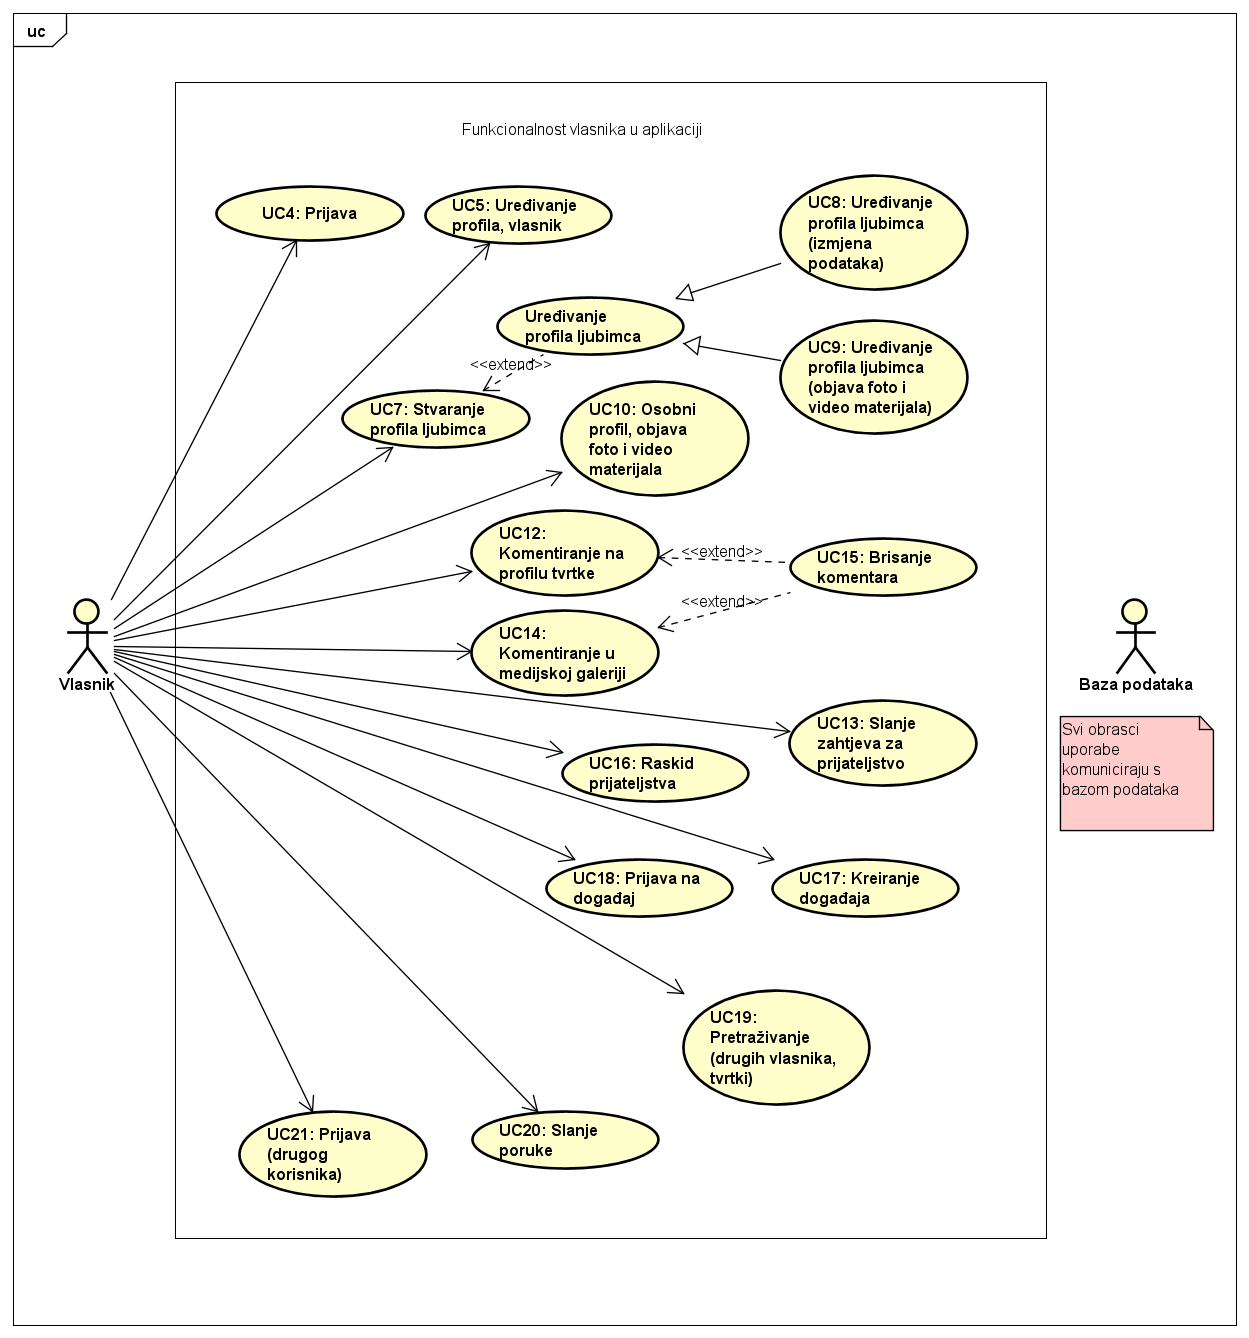
\includegraphics[width=\textwidth]{slike/funkcionalnost_vlasnika.png}
						\caption{Funkcionalnost vlasnika u aplikaciji}
					\end{figure}
					\begin{figure} 
						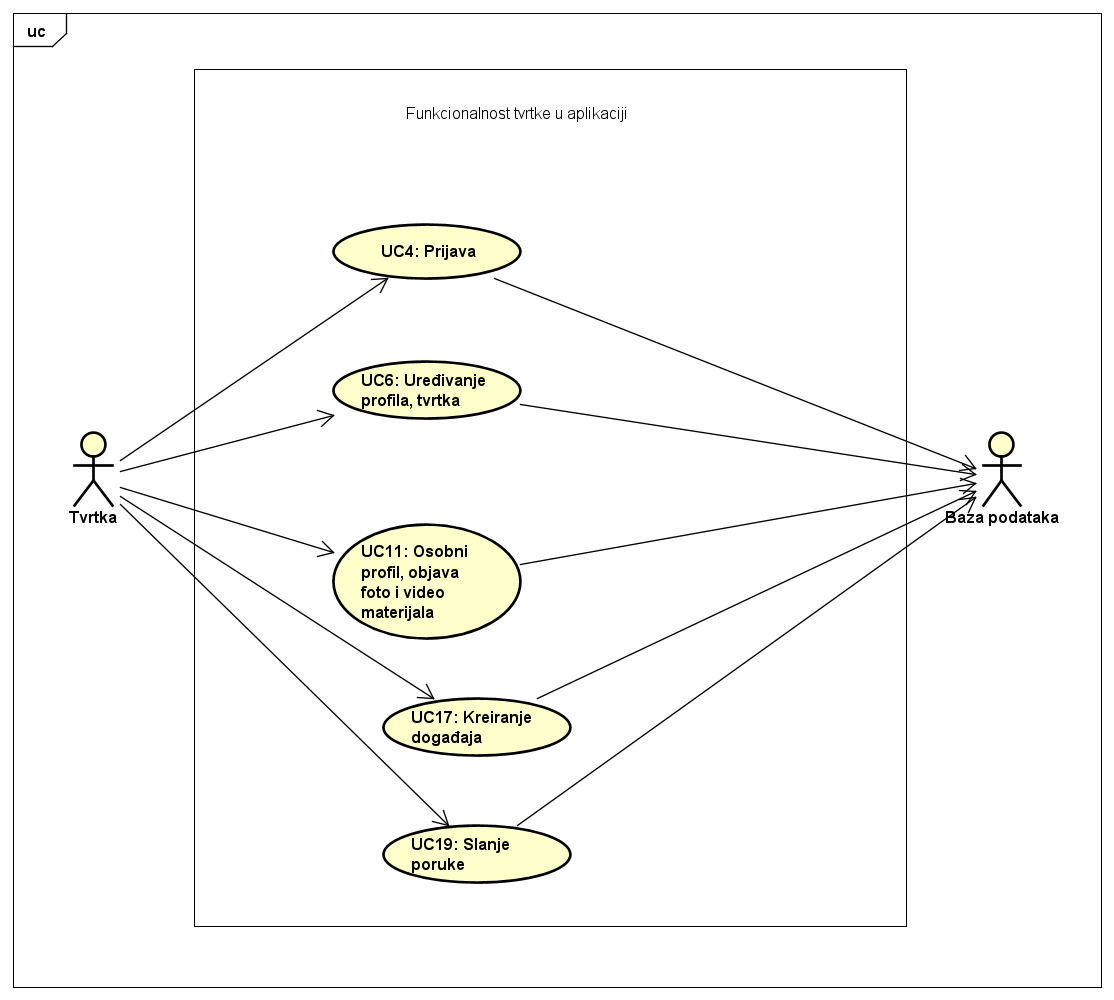
\includegraphics[width=\textwidth]{slike/funkcionalnost_tvrtke.png}
						\caption{Funkcionalnost tvrtke u aplikaciji}
					\end{figure}
					\begin{figure} 
						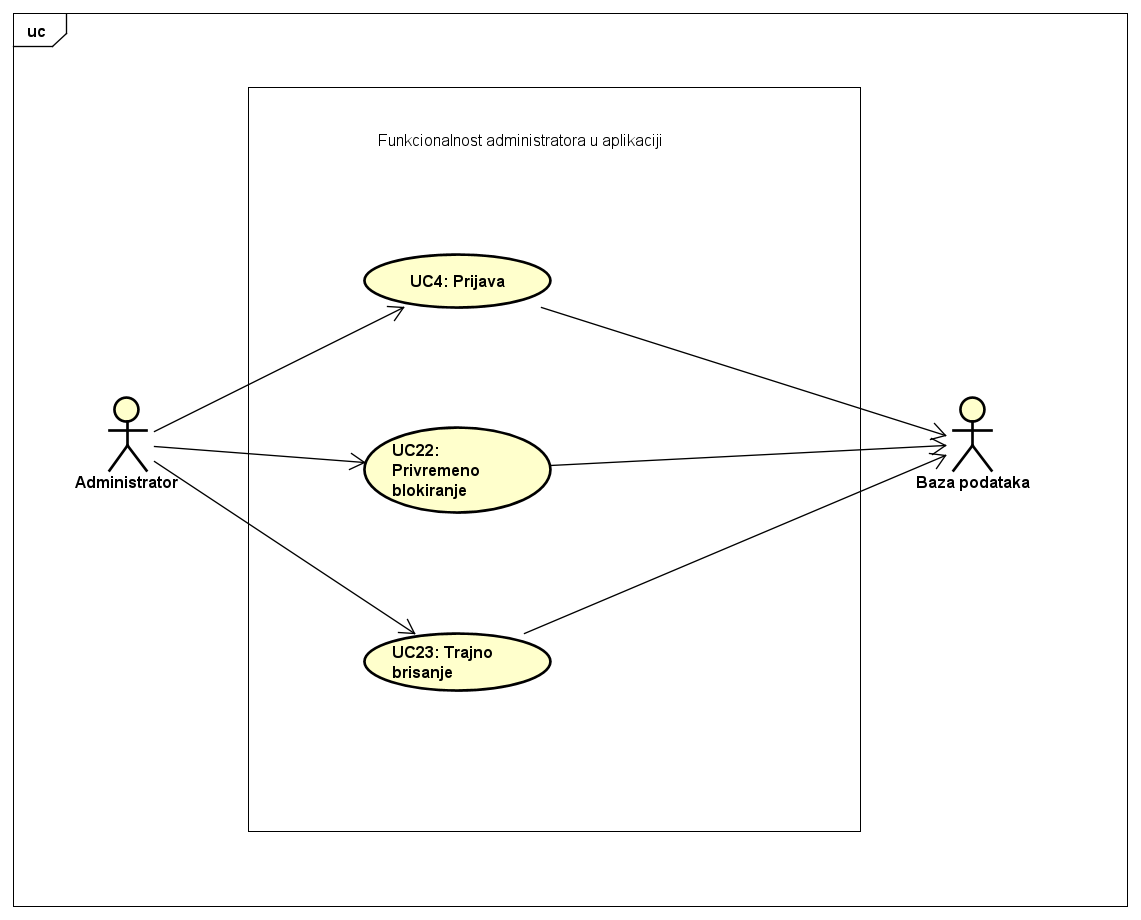
\includegraphics[width=\textwidth]{slike/funkcionalnost_administratora.png}
						\caption{Funkcionalnost administratora u aplikaciji}
					\end{figure}
				\eject		
				
			\subsection{Sekvencijski dijagrami}
				
				\textbf{Obrazac uporabe UC7 - Stvaranje profila ljubimca}\\
				\indent Vlasnik u aplikaciji odabire opciju stvaranja profila ljubimca. Otvara mu se prazan obrazac za kreiranje profila koji vlasnik ispunjava i prosljeđuje aplikaciji koja sprema podatke u bazu podataka i tako je stvoren novi profil ljubimca.
				
				\begin{figure}[H]
					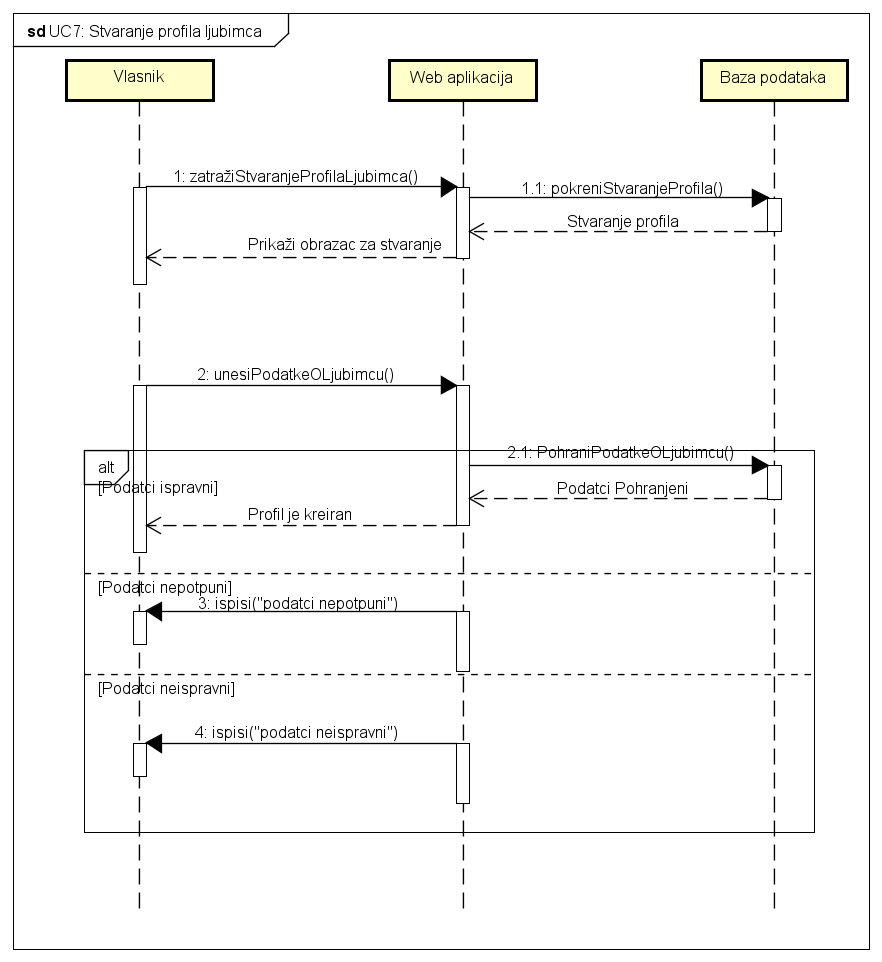
\includegraphics[scale=0.5]{slike/UC7.PNG} %veličina slike u odnosu na originalnu datoteku i pozicija slike
					\centering
					\caption{Sekvencijski dijagram za UC7}
				\end{figure}
				
				\pagebreak
				\textbf{Obrazac uporabe UC16 - Kreiranje događaja}\\
				\indent Tvrtka u aplikaciji odabire opciju kreiranja novog događaja. Otvara se obrazac za kreiranje novog događaja koji se ispunjava i prosljeđuje aplikaciji koja pohranjuje podatke u bazu podataka i kreira se novi događaj
				
				\begin{figure}[H]
					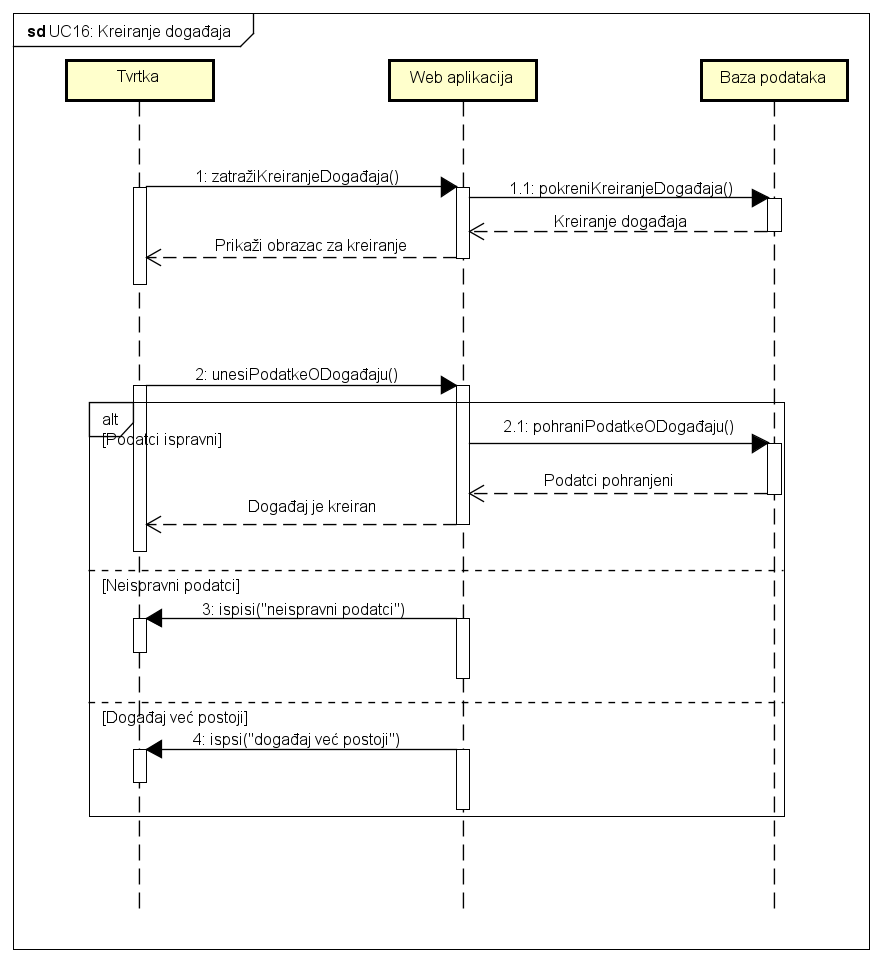
\includegraphics[scale=0.5]{slike/Uc16.PNG} %veličina slike u odnosu na originalnu datoteku i pozicija slike
					\centering
					\caption{Sekvencijski dijagram za UC17}
				\end{figure}
				
				\pagebreak
				\textbf{Obrazac uporabe UC18 - Prijava na događaj}\\
				\indent Vlasnik u aplikaciji odabire opciju prijave na događaj. Nakon odabira željenog događaja vlasnik potvrđuje prijavu i podatci se spremaju u bazu podataka. Vlasnik je prijavljen na odabrani događaj.
				
				\begin{figure}[H]
					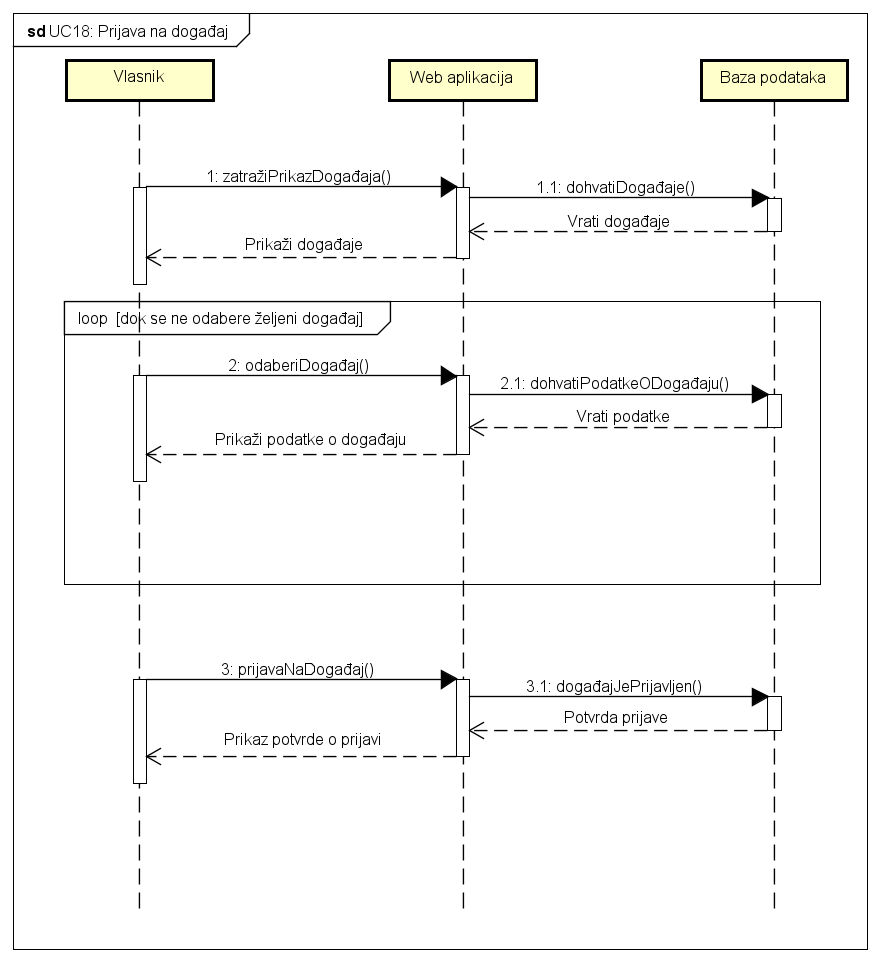
\includegraphics[scale=0.5]{slike/UC18.PNG} %veličina slike u odnosu na originalnu datoteku i pozicija slike
					\centering
					\caption{Sekvencijski dijagram za UC18}
				\end{figure}
				
				\pagebreak
				\textbf{Obrazac uporabe UC22 - Trajno brisanje}\\
				\indent Administrator u aplikaciji odabire željenog korisnika kojeg želi trajno obrisati. Potvrdom na brisanje korisnika svi njegovi podatci o računu se brišu iz baze podataka i korisnik se više ne može prijaviti u aplikaciju.
				
				\begin{figure}[H]
					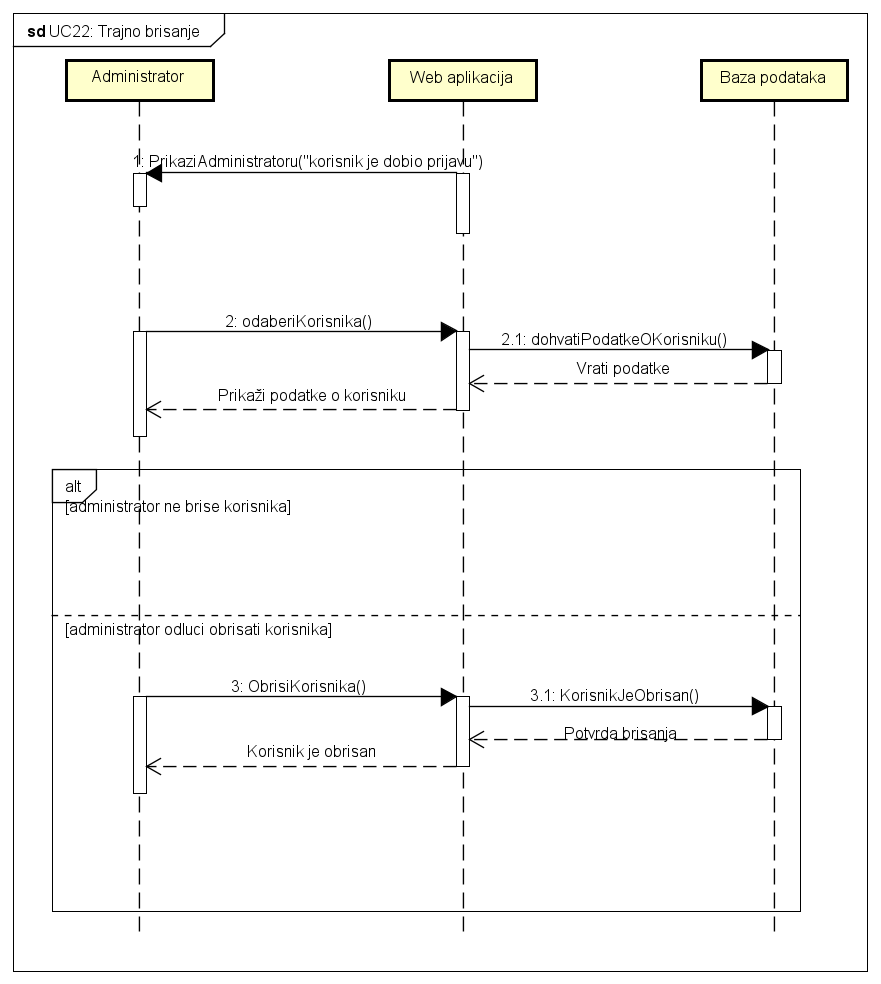
\includegraphics[scale=0.5]{slike/Uc22.PNG} %veličina slike u odnosu na originalnu datoteku i pozicija slike
					\centering
					\caption{Sekvencijski dijagram za UC23}
				\end{figure}
				
				
				\eject
	
		\section{Ostali zahtjevi}
				\begin{packed_item}
					\item Sustav mora podržavati rad za dovoljno korisnika istovremeno
					\item Korisničko sučelje i sustav moraju podržavati hrvatske znakove
					\item Upiti bazi podataka moraju čekati najviše 3 sekunde
					\item Sustav treba biti jednostavan i intuitivan za korištenje
					\item Sustav mora poštovati načelo nadogradnje uz minimalnu promjenu
					\item Veza s bazom podataka mora biti zaštićena, brza i otporna na vanjske greške
					\item Podaci se moraju sanirati prije slanja bazi podataka
				\end{packed_item}
			 
			 
			 
	